\section{Availability}

Availability measures the delivery of correct service as a fraction of the time that the system is ready to provide a service. 
\\
%A system is an entity that interacts with other entities, which constitute the environment of the system and
%can be other systems, humans or the physical world \cite{1335465}. Fundamental properties of communication systems
%are \textit{functionality, performance, security and dependability}. 
The services provided by the system through it's service interface to the user(s) 
is described by the functional specification. Whenever the provided service
deviates from correct service a system failure, called \textit{outage} or \textit{downtime}\footnote{in contrast, \textit{uptime} does not guarantee correct
service - for example, a server can be 'up' but unreachable} occurs. A failure is defined to be caused originally by a fault inside the system, which may be 
dormant. Under special conditions, the fault \textit{may} become apparent and lead to an error. Faults can be categorized into random and systematic faults:
random faults are unpredictable and concern hardware: for example, because of aging, a memory cell can be damaged, but the fault may be hidden because the cell
is not used. Software and design faults belong to systematic faults. Similar to the damaged memory cell, a software bug may only 
trigger an error under special inputs. In both cases, the error then causes a deviation from the required operation of the system or a subsystem. Finally, the 
error can cause a failure if the system fails to provide the correct service.
\\
Availability is measured subjectively from the system user's point of view.
While an optimal system may have availability of 1, this value is only of theoretical value because random faults can not be ruled out. Therefor,
system failures are inevitable, and availability is often given in \textit{x-9s}\footnote{read 'one-nine', 'two-nines', ...} notation, denoting the 
number of nines in the time fraction the system delivers correct service, as shown in table \ref{table:x-9}.
The availability is normally asserted by the provider of the system to the customer by an
\gls{sla} - if the \gls{sla} is violated, the provider may be fined.
\begin{figure}
    \centering
    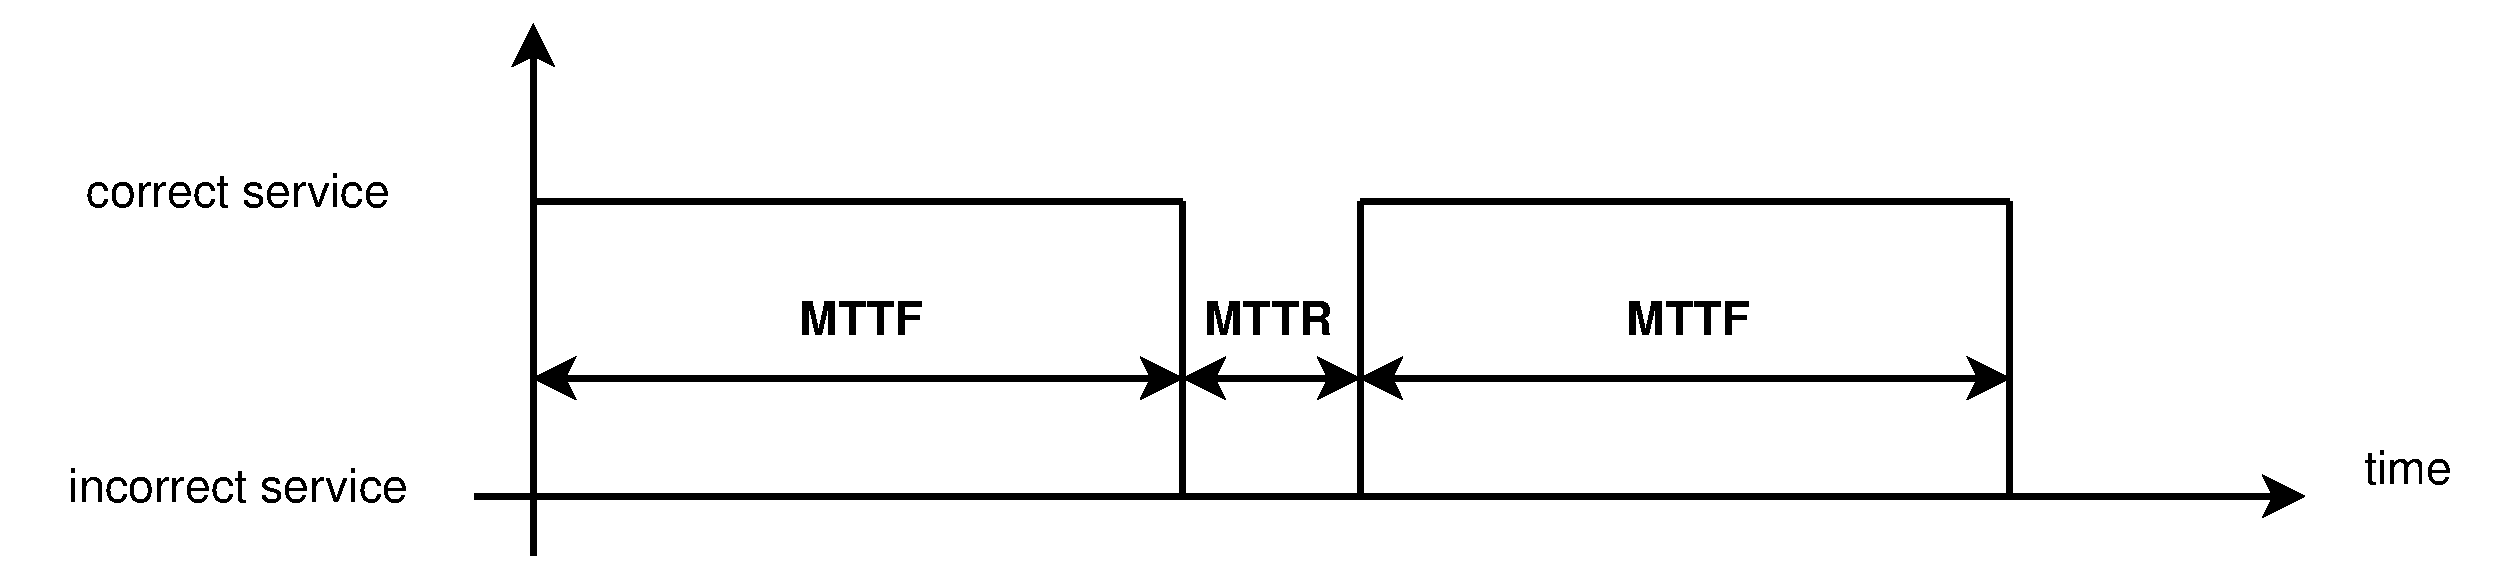
\includegraphics[width=1\textwidth]{figures/availability}
    \caption{Relationship between \gls{mttf} and \gls{mttr}}
    \label{fig:relmttfmttr}
\end{figure}
\begin{center}
\begin{tabular}{ c | c c  }
 \label{table:x-9}
  x & $P_{availability}$ & failure duration per year \\ \hline
  1 & 90,0000    & ~ 36 days \\
  2 & 99,0000    & ~ 3,5 days  \\
  3 & 99,9000    & ~ 9 hours \\
  4 & 99,9900    & ~ 1 hour \\
  5 & 99,9990    & ~ 5 minutes \\
  6 & 99,9999    & ~ 31 seconds \\ 
  
\end{tabular}
\end{center}
For a system with 6-9 availability, this would mean that the system provider assures that the system will be unavailable not more than about 31 seconds over a
whole year.
\\
\\
Availability is important simply because unavailable systems cause costs. Because of the relation of availability to reliability and the maintainability
of the system, as shown in equation \ref{EQUavailability} and figure \ref{fig:relmttfmttr}, two options to improve availability exist: either increasing
the \gls{mttf} (i.e. increasing reliability) or decreasing \gls{mttr}.
%An informal definition of a dependable system is a system which delivers a service that can be justifiable trusted. More formally,
%dependability consists of the following attributes:
%\textit{Availability}, which means that the system is ready for correct service, \textit{reliability}, the continuity of correct service,
%\textit{safety}, i.e. the avoidance of catastrophic consequences \textit{integrity}, s.t. the system cannot be modified in an unwanted manner
%and \textit{maintainability}, so that the system can be repaired in the case of a failure.
%In case of a secure system, another important property is \textit{confidentiality}, which means that no information is disclosed to unauthorized 
%entities.
\begin{align}\label{EQUavailability}
 P_{Availability} = \frac{t_{correct\ service}}{t_{total}} =  \frac{{\gls{mttf}}}{\gls{mttf}+\gls{mttr}}
\end{align}
Reliability measures the probability that the service will work as expected until time $t$:
\begin{align}\label{expFailLaw}
 R(t) = e^{-\lambda(t-t_0)}
\end{align}
\ref{expFailLaw} is known as the \textit{exponential failure law}, $\lambda$ denotes the failures per hour, it's inverse $\frac{1}{\lambda}$ is
called \gls{mttf}. Reliability can also be expressed in terms of \textit{un}reliability, denoted $Q(t)$:
\begin{align}
 Q(t) = 1 - R(t)
\end{align}
Maintainability measures the time that is needed to repair a system, with $\mu$ denoting the repair rate and $\frac{1}{\mu}$ called \gls{mttr}.
\\
\\
\gls{ha} characterizes a system that is designed in a way to avoid outages, or in case of a failure that can be repaired in shortest possible time. 
The level of the needed availability depends on the environment of the system and must be weighted against the additional costs, introduced by improving availability.
Therefor, no hard definition for \gls{ha} can be given - it is a design goal and depends on the context. Availability requirements will most certainly be higher
for systems in safety-critical requirements. A safety-critical system must not fail, otherwise endangering human lives or 
causing substantial economic loss or environmental damage \cite{1007998}.
On the other side, systems that will produce only minor costs when not operating correctly
will maybe have to meet less stringent availability levels.
\\
For example, our society heavily depends on electric power supply, an outage
is nearly unacceptable. On the other side, it is impossible to guarantee 100\% availability, so \textit{if} a power outage occurs, the system must be fixed as soon as
possible to restore correct service, otherwise risking human lives. On the contrary, a booking system will obviously result in financial losses for the company 
if not working, but no more serious consequences are to be assumed.
\\
\\
This work's focus lies on security-critical systems, trying to increase availability of KNX networks, but restricting it's deployment to
environments without safety-critical needs. Thus, safety criticality is neglected here because of it's most stringent demands, as needed in avionics
or weapons systems.
The difference between safety-critical and security-critical systems can be given as follows \cite{5784222}: safety means that software must not be harm the 
world (i.e. containment), while security means that the world must not harm software (i.e. protection). 
\\
\\
Every system will most likely consist of different and distinct components, each with it's own reliability and failure rates. Finally, the system
will possess an overall reliability, determining it's availability. To model the resulting system, the components will be put together in a mixture of
serial and parallel systems.
\begin{figure}
    \centering
    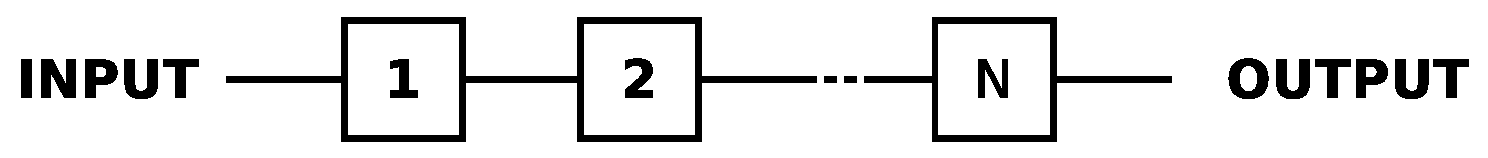
\includegraphics[width=0.8\textwidth]{figures/seriesSystem.eps}
    \caption{Model of a series system}
    \label{fig:serSys}
\end{figure}
For example, if all $i$ components, ranging from $1$ to $N$, are necessary to work correctly for the overall system to deliver correct service, this can be modeled as
a series system, see figure \ref{fig:serSys}. This does not mean that the components are necessarily connected in a serial way, it just stresses that failure
of one single components breaks the whole system. System's reliability equals the product of all component's reliabilities:
\begin{align}
R_{system}(t) = \prod_{i=1}^{N} R_{i}(t) 
\end{align}
\\
\\
In contrast, a system containing redundant components, failure of one such component must not produce an outage of the overall system. This can be modeled as
a parallel system \ref{fig:parallelSys}. Here, the overall reliability can be calculated as given in \ref{parallelSysEqu}.
\begin{figure}
    \centering
    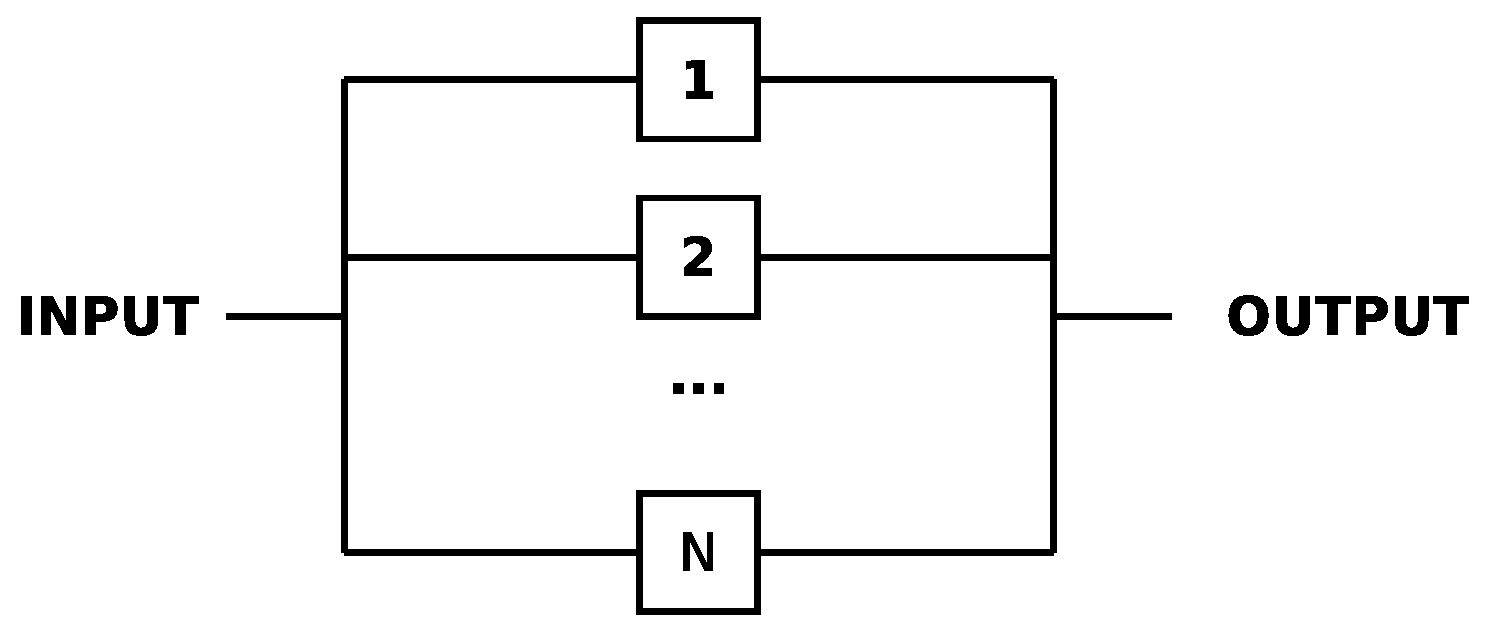
\includegraphics[width=0.8\textwidth]{figures/parallelSys.eps}
    \caption{Model of a parallel system}
    \label{fig:parallelSys}
\end{figure}

\begin{align}\label{parallelSysEqu}
 R(t)_{system} = 1 - \prod_{i=1}^{N} 1- R_{i}(t) = 1 - \prod_{i=1}^{N} Q_{i}(t)
\end{align}
Mixed systems, containing paralell and series system, can be calculated by iteratively condensing serial- or parallel subsystems into single components,
as shown in figure \ref{fig:mixedSys}.
\begin{figure}
    \centering
    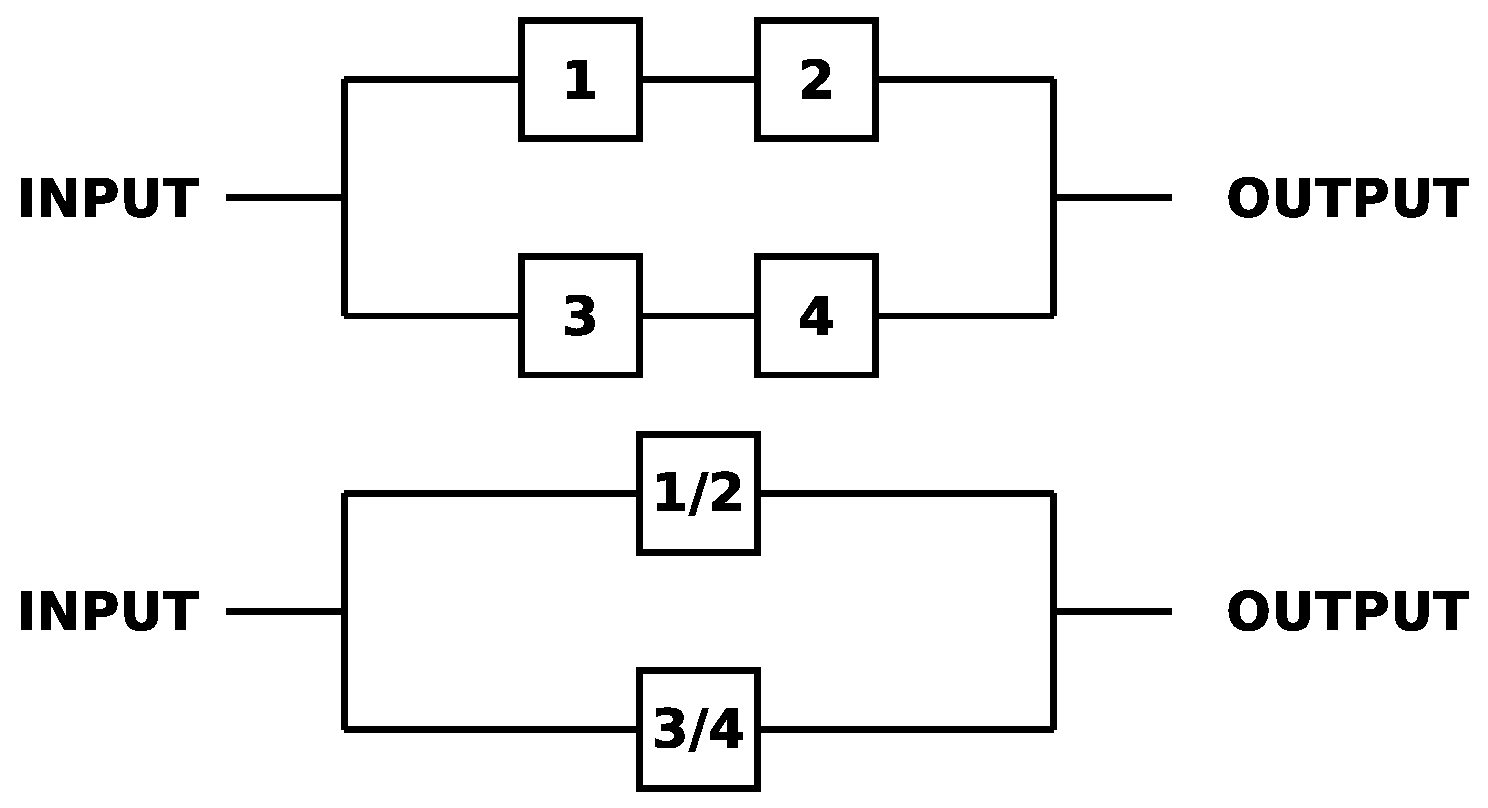
\includegraphics[width=0.8\textwidth]{figures/mixedSys.eps}
    \caption{Condensing a mixed system}
    \label{fig:mixedSys}
\end{figure}
\\
\\
Examining parallel system, it is clear that usage of redundant devices can improve availability, with the paradox situation that adding components also adds
complexity and can therefor worsen reliability and availability.


MARKOV model??